\documentclass[11pt]{article}

\usepackage{float} % [H] option for tables
\usepackage{booktabs} % table ruling
\usepackage{framed} % Frame for listings
\usepackage{fullpage} % Use the full page
\usepackage{color}
\usepackage{tikz}
\usepackage{matlab-prettifier} % Matlab
\setlength\parindent{0pt} % No indentation


% Headers
\usepackage{fancyhdr}
\setlength{\headheight}{15.2pt}
\pagestyle{fancy}
\setlength\headsep{30pt}
\lhead{Youssef Beltagy and Samuel Hunter}   					%  Your name on the left header.
\chead{\textsc{Lab 3}}			%  Title in the center.
\rhead{\today}							%  Date on the right header.

% Matlab blocks
\lstset{
  style              = Matlab-editor,
  basicstyle         = \mlttfamily,
  mlshowsectionrules = true,
  escapeinside={//}{\^^M},
}

% Cover Page Settings
\title{
    \textsc{Lab 3 Report: Fourier Series and Gibbs Phenomenon}
}

\author{
    \Large{Youssef Beltagy and Samuel Hunter} \\
    \large \textsc{AUT21 BEE 235}
}

\date{\today}



%--------------------------------------------
%%%%%%%%%%%%%%%%%%%%%%%%%%%%%%%%%%%%%%%%%%%%%%%%%%%%
% END OF THE PREAMBLE AND BEGINNING OF THE ACTUAL DOCUMENT
%%%%%%%%%%%%%%%%%%%%%%%%%%%%%%%%%%%%%%%%%%%%%%%%%%%%
%--------------------------------------------

\begin{document}


\maketitle % Make the cover page
\pagebreak


\section{Abstract}


Part 1 of this lab introduces the concept of additive synthesis.
We load a pre-recorded trumpet sound signal, and apply a Fourier transform to find the magnitudes and frequencies of 10 peak harmonics.
We then take these values to sum together 10 sine functions, synthesizing a new sound signal that sounds like the pre-recorded sample.


We experiment with fourier series signal synthesis and
observe the limitations of this technique.

% =================================================
% PART 1
% =================================================
\section{Part 1 --- Signal Synthesis}

After loading and plotting the pre-recorded trumpet sound signal onto a graph, I measured the coordinates of two different peaks:

\begin{table}[H]
	\centering
	\begin{tabular}{cccc}\toprule
		Peak No. 1 & Peak No. 2 & Period (\# of samples) & $F_0 (Hz) = F_s / (\textrm{\# of samples})$ \\\midrule

		$X_1 = 70, Y_1 = 0.99969$ &
		$X_2 = 112, Y_1 = 0.99969$ &
		$|X_2-X_1| = 42$ &
		$F_0 = 11025 / 42 = 262.5\;Hz$ \\\bottomrule
	\end{tabular}
	\caption{\label{tab:two-peaks}Two sampled peaks of the trumpet sound signal}
\end{table}

The difference between the two peaks were 42 samples.
With a sample rate of $F_s = 11025\;sample*Hz$, the difference is $262.5\;Hz$.
I then applied a Fourier transform on the trumpet signal, and measured the magnitudes and frequency of the first seven harmonic peaks:

\begin{table}[H]
	\centering
	\begin{tabular}{rrr}\toprule
		Harmonic & Magnitude & Frequency (Hz) \\\midrule

		1 & 11.795 & 258.398 \\
		2 & 37.749 & 538.33  \\
		3 & 65.114 & 796.729 \\
		4 & 52.244 & 1055.13 \\
		5 & 59.593 & 1335.06 \\
		6 & 38.994 & 1593.46 \\
		7 & 28.305 & 1851.86 \\\bottomrule
	\end{tabular}
	\caption{\label{tab:first-harmonics}7 first harmoncs}
\end{table}

The differences of these peaks were 279.93, 258.40, 258.40, 279.93, 261.40, and 258.40 Hz.
The mean of these differences is 265.93 Hz (1.3\% difference), and the median of these differences is 258.40 Hz (1.6\% difference), so the data aligns well with the difference of peaks I measured previously.

To synthesize a new trumpet signal, I recorded the 10 strongest (in magnitude) harmonic peaks:

\begin{table}[H]
	\centering
	\begin{tabular}{c c c}\toprule
		Peak & Magnitude & Frequency (Hz) \\\midrule

		 1 & 65.114 & 796.729 \\
		 2 & 59.593 & 1335.06 \\
		 3 & 52.244 & 1055.13 \\
		 4 & 38.994 & 1593.46 \\
		 5 & 37.749 & 538.33  \\
		 6 & 28.305 & 1851.86 \\
		 7 & 15.724 & 2390.19 \\
		 8 & 15.208 & 2648.58 \\
		 9 & 12.487 & 2110.25 \\
		10 & 11.795 & 258.398 \\\bottomrule
	\end{tabular}
	\caption{\label{tab:strongest-harmonics}10 strongest harmonic peaks}
\end{table}

I then created a matlab script that summed up 10 sine waves into a $2*F_s$-long vector to synthesize a 2-second long trumpet signal:

% Synthesis code
\begin{framed}
	\lstinputlisting[caption=Signal synthesis code]{signal_synthesis.m}
\end{framed}

% Synthesis output
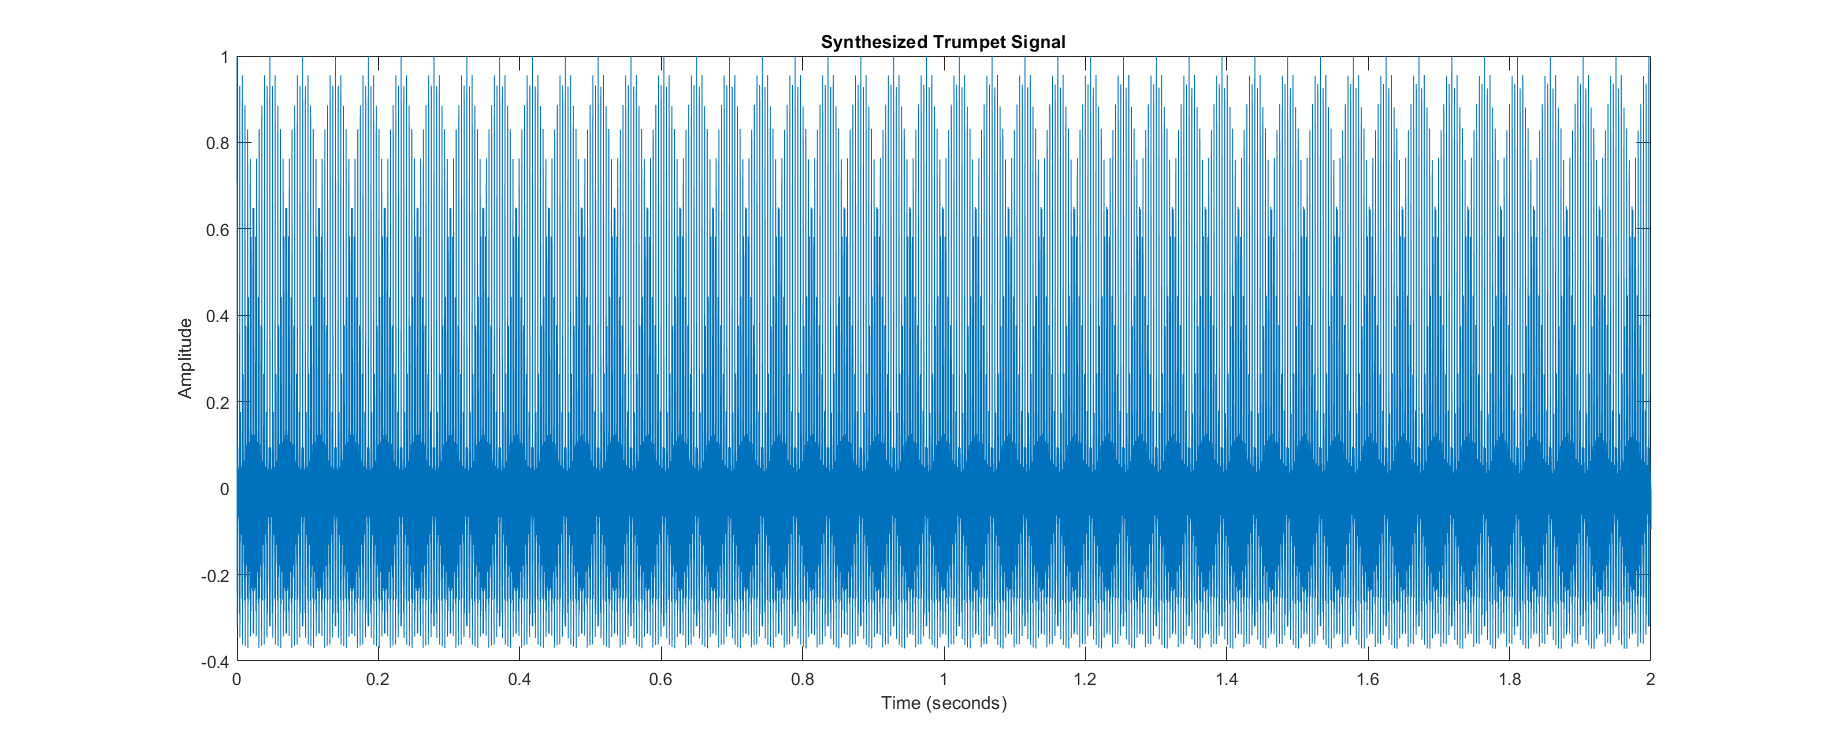
\includegraphics[scale=1.0]{signal_synthesis.png}

The audio generated sounded much like the pre-recorded trumpet signal.
The main difference is that the synthesized signal has zero variance in tone.

% =================================================
% PART 2
% =================================================
\pagebreak
\section{Part 2 --- Fourier Series Approximation of a Square Wave}

In this section, we synthesized a square wave signal using a fourier series.
When the number of coefficients is low, the synthesized signal displays the Gibbs
phenomenon where the signal overshoots and undershoots at sharp transitions.

\subsection{C\_k Phase and Magnitude}

We generated and plotted the C\_k coefficients of the fourier series
we used to synthesize the square wave.\\

Below you can see the magnitudes and phases of the coefficients.

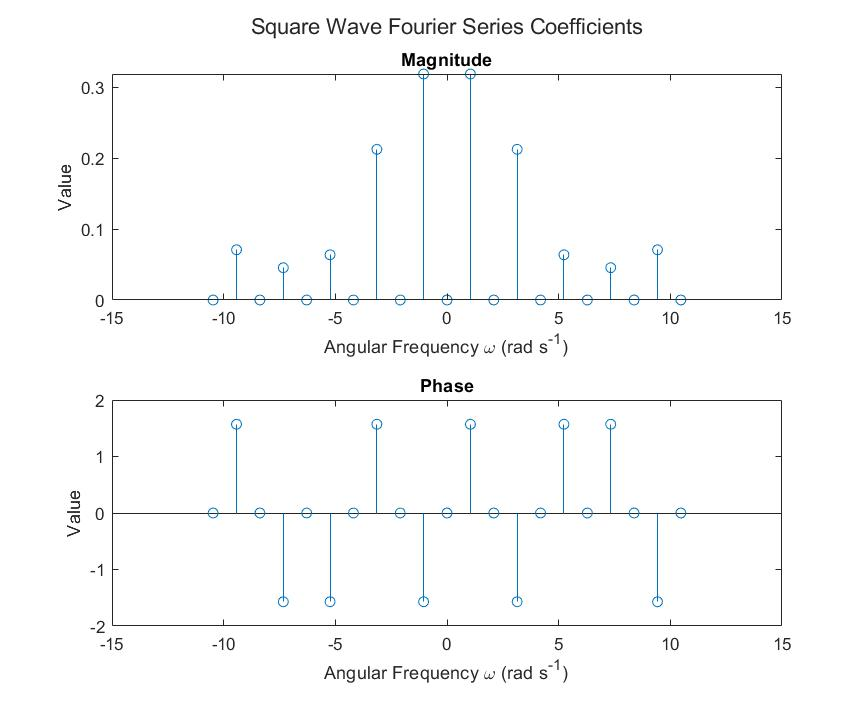
\includegraphics[width=\textwidth]{ck_values.png}

\lstinputlisting{gibbs.m}

\subsection{Square Wave Synthesis}

We developed a function that generates an approximation of a square wave
given the time of the signal and the K\_{max} of the coefficients.

\lstinputlisting{squarewave.m}

\subsection{Square Wave Plots}

We plotted the output from our synthesizing function.

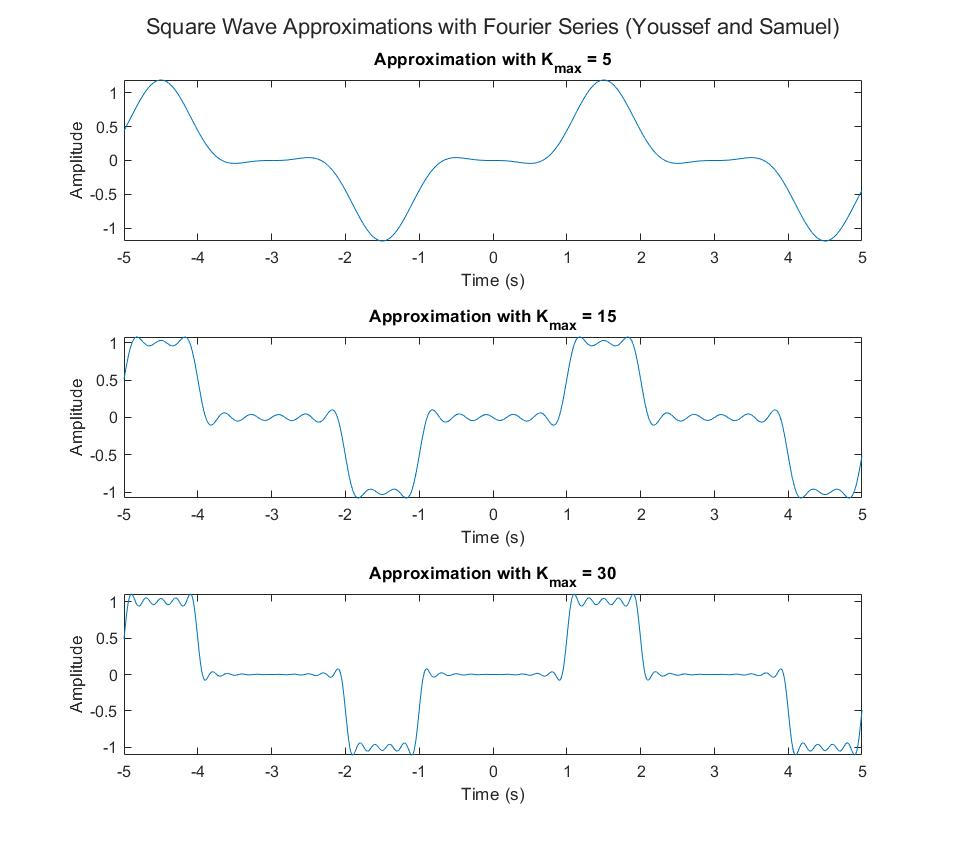
\includegraphics[width=\textwidth]{squarewaves.png}

\lstinputlisting{squarewave_plot.m}

\subsection{Gibbs Phenomenon}

The plots didn't demonstrate the phenomenon enough,
so we wrote a script to generate a video of synthesized signal
as k\_{max} increases.

\lstinputlisting{squarewave_video.m}

When K\_{max} is less than 500, the Gibbs phenomenon is clear.
The signal rings (overshoots and undershoots) at sharp transitions.\\

Between K\_{max} = 400 and K\_{max} = 500, the ringing decreases.
When K\_{max} rises above 500, the Gibbs phenomenon disappears.
After that it appears again; then it disappears again; 
then it appears again, and the process repeats.

\section{Conclusion}

Part 1 demonistrated the use of the Fourier transform to assist in the synthesis of audio signals.
By summing together cosines mapping to the highest-magnitude harmonics in some sample, I can create a function that generates a signal that roughly mimics the timbre of a sound piece.

However, this additive synthesis process alone is not able to replicate any ``wibbly-wobbly'' sound that appears when there's a low-frequency modulation in the sample.
The synthesized trumpet signal demonstrated this inability by having zero variance in tone that the pre-recorded signal had.
Nonetheless, a Fourier transform can no doubt generate sound tables that can be used by synthesizers and other digital audio tools as a base for instruments and other uses for sound.

In this lab, we synthesized a square wave using 
fourier series and observed the Gibbs phenomenon.

\end{document}
